
\thispagestyle{empty}

\vbox{}
\vfill
\vfill
\vfill
\begin{center}
\rule{.9\linewidth}{.2ex}


\includegraphics[width=\linewidth]{scipy2009confs}

\rule{.9\linewidth}{.2ex}

\vfill

{\sffamily\bfseries
{\huge
Proceedings of the 9$^{\text{th}}$ Python in Science Conference}

\bigskip
\large
SciPy Conference -- 
Pasadena, CA, June 28--July 3,
2010. 
}

\vfill
\vfill
\vfill
\hline

Editors: \quad St\'efan {\sc van der Walt}, \quad K. Jarrod {\sc Millman},
\quad Ga\"el {\sc Varoquaux}

\end{center}
\vfill
\vfill
\vfill
%\hfill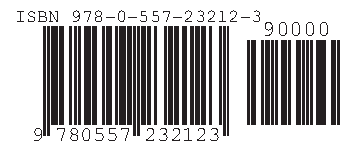
\includegraphics[width=.3\linewidth]{isbn_barcode}
%\vbox{}

\pagebreak

\thispagestyle{empty}

\cleardoublepage 

\setcounter{page}{0}
\vbox{}
\vfill
\thispagestyle{empty}
\tableofcontents
\vfill

{\small
	The content of the articles of the {\sl Proceedings of the Python in
	Science Conference} is copyrighted and owned by their original
	authors.

	For republication or other use of the material published, please
        contact the copyright owners to obtain permission.

    \bigskip
    \hrule


Proceedings of the 9th Python in Science Conference
by St\'efan van der Walt, K. Jarrod Millman, Ga\"el Varoquaux
ISBN:   978-0-557-23212-3

}

\vfill
\vbox{}
\markright{}{}
\markbox{}{}
\clearpage
\thispagestyle{empty}
\section*{Organization}

\def\bfsf{\bfseries\sffamily }

%\hspace*{-.5cm}%
\begin{tabular}{p{3.7cm}p{0.75\textwidth}}
{\bfsf Archive note}&\\
This restored copy omits event staff, institutional affiliations, and personal
contact metadata from the original proceedings template.\\
\end{tabular}

\pagestyle{fancy}
\resethandings
\cleardoublepage 
\markright{}{}
\markbox{}{}
\pagestyle{fancy}
\resethandings

